%\textcolor{red}{\hrulefill \textsc{Unfinished Section}\hrulefill}  \\
As discussed in Section~\ref{sec:detector:beamsbucketsbunches}, the nominal filling scheme results in a proton bunch spacing of 25~ns and so the collision rate is roughly 40 million events every second.
Writing this much data to disk becomes intractable and impractical.
Additionally most collisions produce physically uninteresting events coming from high cross section SM processes and as the gambit here at the LHC is to measure ultra rare processes there is no love lost. 
The goal then is to select the ``most interesting'' events to be saved at the highest rate possible.
This is what is defined as the \emph{Trigger}.
Computational resources ultimately become the limiting factor (as physicists would keep every event if they could just to have them) resulting in an upper limit of 2000 events per second being able to be saved at ATLAS.
ATLAS specifically has a two-level trigger system \cite{ATLAS:2016wtr} used to select events.
The first-level trigger is implemented in hardware (referred to often as ``online'' or Level 1 (L1)) and uses a subset of the detector information to reduce the accepted rate to a maximum of about 100 kHz.
This is followed by a software-based trigger (referred to often as ``offline'' or the High Level Trigger (HLT)) that reduces the accepted event rate to 1 kHz on average, depending on the data-taking conditions.
In Figures \ref{fig:detector:L1rate} and \ref{fig:detector:HLTrate} the L1 and HLT trigger rates are shown for a typical fill in the 2018 data taking period. 
As is apparent in the figures the rate falls off rapidly over time during a fill, as the number of protons per bunch decreases and the emittance (transverse spread of protons) increases.
\begin{figure}[htb]
\makebox[\textwidth][c]{
    \centering
    \begin{subfigure}[b]{0.55\textwidth}
      \centering
      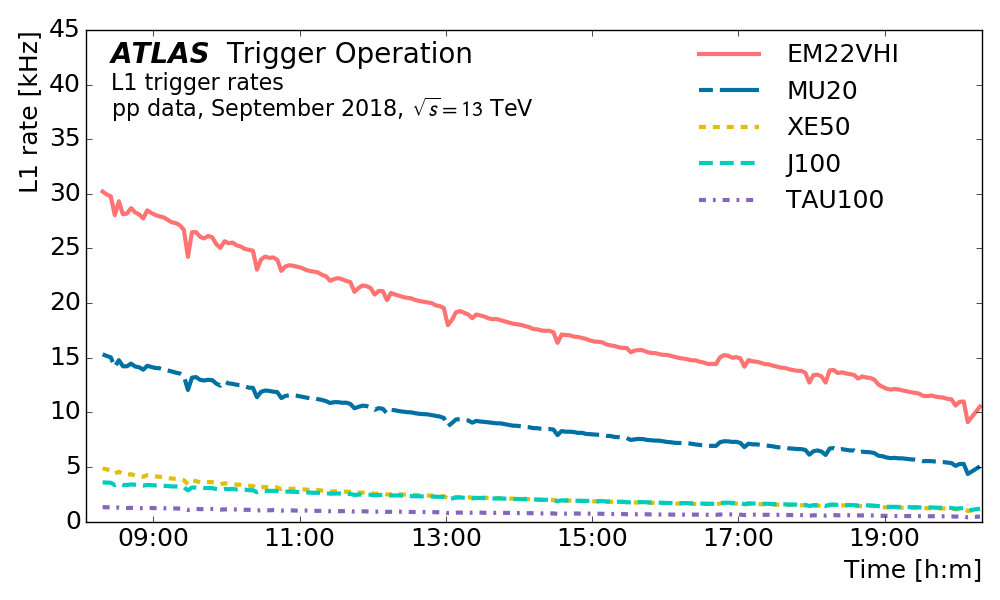
\includegraphics[width=1.0\textwidth]{figs/detector/L1rate.png}
      \caption{}
      \label{fig:detector:L1rate}
    \end{subfigure}
    \hfill
    \begin{subfigure}[b]{0.55\textwidth}
      \centering
      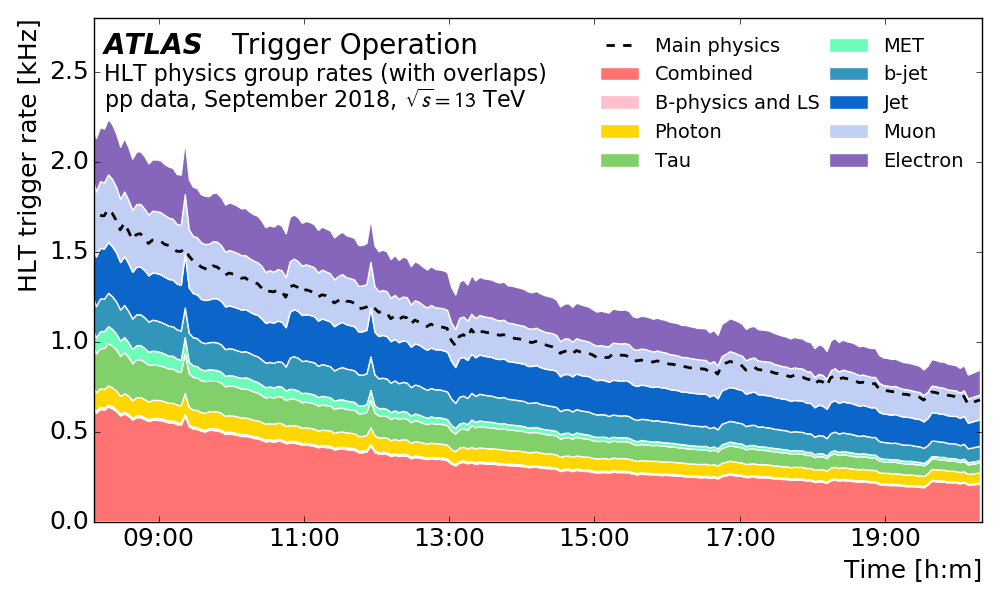
\includegraphics[width=1.0\textwidth]{figs/detector/HLTrate_2018.png}
      \caption{}
      \label{fig:detector:HLTrate}
    \end{subfigure}
}
  \caption[L1 and HLT trigger rates]
          {(a) L1 rates of some representative single-object trigger items, which have not been prescaled.
          These trigger items are based on such objects as electromagnetic clusters (EM), muon candidates (MU), jet candidates (J), missing transverse energy (XE) and tau candidates (TAU).
          The number in the trigger name denotes the trigger threshold in GeV.
          The letters following the threshold values refer to details of the selection: variable thresholds (V), hadronic isolation (H), and electromagnetic isolation (I). 
          (b) HLT trigger rates for different targeted physics processes as a function of time.
          Each of the groups (colors) contains single-object and multi-object triggers.
          The combined group represents multiple triggers of different objects, as combinations of electrons, muons, taus, jets and missing transverse energy
          Overlap between groups is only accounted for in the total main physics stream rate ~\cite{Triggerrates}}
      \label{fig:detector:triggerrates}
\end{figure}
